\documentclass[border=5pt]{standalone}
\usepackage[utf8]{inputenc}
\usepackage{tikz}
\usetikzlibrary{arrows.meta, positioning, shapes.geometric, fit, calc, decorations.pathreplacing}
\usepackage{amsmath}

\definecolor{gcncolor}{RGB}{70,130,180}
\definecolor{adaptivecolor}{RGB}{220,80,60}
\definecolor{entropycolor}{RGB}{60,179,113}
\definecolor{clusterA}{RGB}{100,149,237}
\definecolor{clusterB}{RGB}{255,127,80}
\definecolor{clusterAB}{RGB}{255,200,50}
\definecolor{bglight}{RGB}{248,249,250}
\definecolor{graytext}{RGB}{100,100,100}

\begin{document}
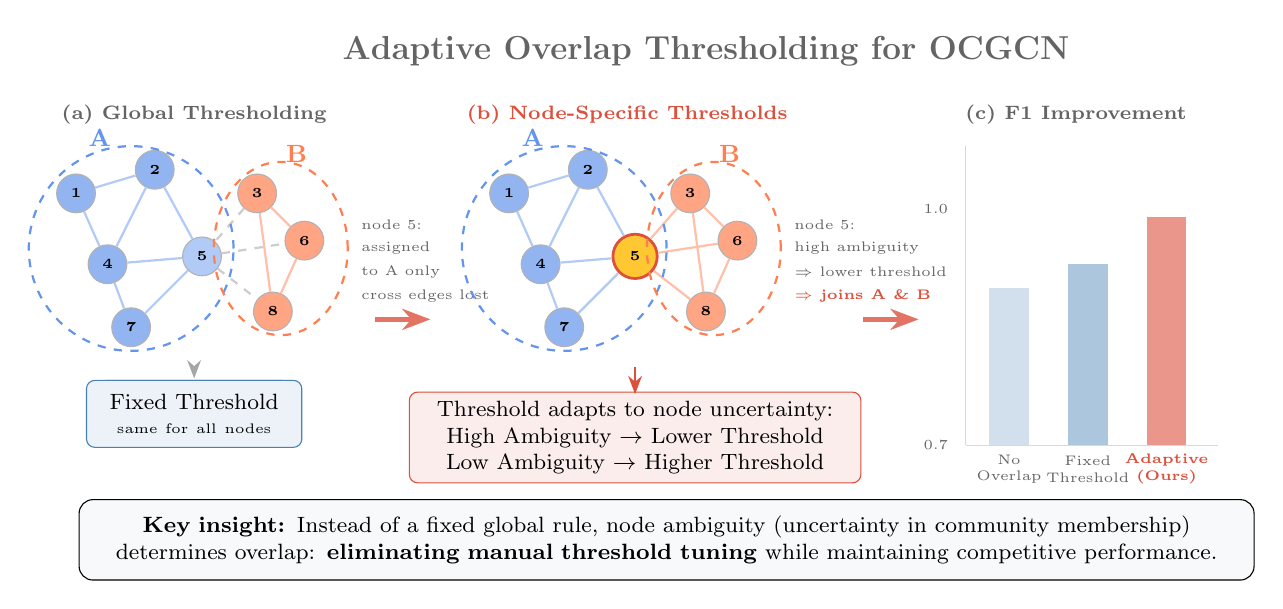
\begin{tikzpicture}[
    >=Stealth,
    node distance=0.8cm,
    every node/.style={font=\small},
    block/.style={draw, rounded corners=3pt, minimum height=0.85cm, align=center, font=\footnotesize},
    vnode/.style={circle, draw=gray!60, minimum size=14pt, inner sep=0pt, font=\tiny\bfseries},
    arrow/.style={->, thick, gray!70},
    bigarrow/.style={->, ultra thick, adaptivecolor!80},
]

% ─── Title ───
\node[font=\bfseries\large, graytext] at (8.5, 6.0) {Adaptive Overlap Thresholding for OCGCN};

% ════════════════════════════════════════════════════════════════════
% PANEL A: Original OCGCN — CRISP
% ════════════════════════════════════════════════════════════════════
\node[font=\bfseries\scriptsize, graytext] at (2.0, 5.2) {(a) Global Thresholding};

\node[vnode, fill=clusterA!70] (p1) at (0.5, 4.2) {1};
\node[vnode, fill=clusterA!70] (p2) at (1.5, 4.5) {2};
\node[vnode, fill=clusterA!70] (p4) at (0.9, 3.3) {4};
\node[vnode, fill=clusterA!70] (p7) at (1.2, 2.5) {7};

\node[vnode, fill=clusterB!70] (p3) at (2.8, 4.2) {3};
\node[vnode, fill=clusterB!70] (p6) at (3.4, 3.6) {6};
\node[vnode, fill=clusterB!70] (p8) at (3.0, 2.7) {8};

\node[vnode, fill=clusterA!50, minimum size=14pt] (p5) at (2.1, 3.4) {5};

\draw[clusterA!50, thick] (p1) -- (p2);
\draw[clusterA!50, thick] (p1) -- (p4);
\draw[clusterA!50, thick] (p2) -- (p4);
\draw[clusterA!50, thick] (p4) -- (p7);
\draw[clusterA!50, thick] (p2) -- (p5);
\draw[clusterA!50, thick] (p4) -- (p5);
\draw[clusterA!50, thick] (p5) -- (p7);

\draw[clusterB!50, thick] (p3) -- (p6);
\draw[clusterB!50, thick] (p6) -- (p8);
\draw[clusterB!50, thick] (p3) -- (p8);

\draw[gray!40, thick, dashed] (p3) -- (p5);
\draw[gray!40, thick, dashed] (p5) -- (p6);
\draw[gray!40, thick, dashed] (p5) -- (p8);

\draw[clusterA, dashed, line width=0.8pt] (1.2, 3.5) ellipse (1.3cm and 1.3cm);
\draw[clusterB, dashed, line width=0.8pt] (3.1, 3.5) ellipse (0.85cm and 1.1cm);

\node[block, fill=gcncolor!10, draw=gcncolor, text width=2.2cm] at (2.0, 1.4) {WMC = 0.30\\[-1pt]{\tiny same for all nodes}};

\draw[arrow] (2.0, 2.0) -- (2.0, 1.85);

\node[font=\small\bfseries, clusterA] at (0.8, 4.9) {A};
\node[font=\small\bfseries, clusterB] at (3.3, 4.7) {B};

\node[font=\tiny, graytext, anchor=west] at (4, 3.8) {node 5:};
\node[font=\tiny, graytext, anchor=west] at (4, 3.5) {assigned };
\node[font=\tiny, graytext, anchor=west] at (4, 3.2) {to A only};
\node[font=\tiny, graytext, anchor=west] at (4, 2.9) {cross edges lost};

\node[block, fill=gcncolor!10, draw=gcncolor, text width=2.5cm] at (2.0, 1.4) {Fixed Threshold\\[-1pt]{\tiny same for all nodes}};
% ════════════════════════════════════════════════════════════════════
% PANEL B: Adaptive — OVERLAP
% ════════════════════════════════════════════════════════════════════
\node[font=\bfseries\scriptsize, adaptivecolor] at (7.5, 5.2) {(b) Node-Specific Thresholds};

\node[vnode, fill=clusterA!70] (a1) at (6.0, 4.2) {1};
\node[vnode, fill=clusterA!70] (a2) at (7.0, 4.5) {2};
\node[vnode, fill=clusterA!70] (a4) at (6.4, 3.3) {4};
\node[vnode, fill=clusterA!70] (a7) at (6.7, 2.5) {7};

\node[vnode, fill=clusterB!70] (a3) at (8.3, 4.2) {3};
\node[vnode, fill=clusterB!70] (a6) at (8.9, 3.6) {6};
\node[vnode, fill=clusterB!70] (a8) at (8.5, 2.7) {8};

\node[vnode, fill=clusterAB, draw=adaptivecolor, line width=1pt, minimum size=16pt] (a5) at (7.6, 3.4) {5};

\draw[clusterA!50, thick] (a1) -- (a2);
\draw[clusterA!50, thick] (a1) -- (a4);
\draw[clusterA!50, thick] (a2) -- (a4);
\draw[clusterA!50, thick] (a4) -- (a7);
\draw[clusterA!50, thick] (a2) -- (a5);
\draw[clusterA!50, thick] (a4) -- (a5);
\draw[clusterA!50, thick] (a5) -- (a7);

\draw[clusterB!50, thick] (a3) -- (a6);
\draw[clusterB!50, thick] (a6) -- (a8);
\draw[clusterB!50, thick] (a3) -- (a8);
\draw[clusterB!50, thick] (a3) -- (a5);
\draw[clusterB!50, thick] (a5) -- (a6);
\draw[clusterB!50, thick] (a5) -- (a8);

\draw[clusterA, dashed, line width=0.8pt] (6.7, 3.5) ellipse (1.3cm and 1.3cm);
\draw[clusterB, dashed, line width=0.8pt] (8.6, 3.5) ellipse (0.85cm and 1.1cm);

%% Annotation — shifted left to avoid bar chart
%\node[font=\tiny, graytext, anchor=west] at (9.7, 3.8) {node 5:};
%\node[font=\tiny, graytext, anchor=west] at (9.7, 3.5) {high entropy};
%\node[font=\tiny, graytext, anchor=west] at (9.7, 3.2) {$\Rightarrow$ low WMC$_i$};
%\node[font=\tiny, graytext, anchor=west] at (9.7, 2.9) {$\Rightarrow$ joins A \& B};
%
%% Threshold boxes — wider left box for 3 lines, moved down
%\node[block, fill=entropycolor!10, draw=entropycolor, text width=3.0cm] (entbox) at (6.0, 1.0) {Entropy-Adaptive: $\mathrm{WMC}_i = \mathrm{WMC}_b (1{-}\lambda H_i)$};
%\node[block, fill=adaptivecolor!10, draw=adaptivecolor, text width=3.0cm] (margbox) at (9.2, 1.0) {Margin-Adaptive: $\mathrm{WMC}_i = \mathrm{WMC}_b (1{-}\lambda A_i)$};
%
%\node[font=\bfseries\scriptsize, adaptivecolor] at (7.5, 5.2) {(b) Node-Specific Thresholds};
%
%% اضافه کردن برچسب خوشه ها
\node[font=\small\bfseries, clusterA] at (6.3, 4.9) {A};
\node[font=\small\bfseries, clusterB] at (8.8, 4.7) {B};

% Annotation 
\node[font=\tiny, graytext, anchor=west] at (9.5, 3.8) {node 5:};
\node[font=\tiny, graytext, anchor=west] at (9.5, 3.5) {high ambiguity};
\node[font=\tiny, graytext, anchor=west] at (9.5, 3.2) {$\Rightarrow$ lower threshold};
\node[font=\tiny\bfseries, adaptivecolor, anchor=west] at (9.5, 2.9) {$\Rightarrow$ joins A \& B};

\node[block, fill=adaptivecolor!10, draw=adaptivecolor, text width=5.5cm, align=center] (conceptbox) at (7.6, 1.1) {
  Threshold adapts to node uncertainty:\\ 
  {\footnotesize High Ambiguity $\rightarrow$ Lower Threshold}\\ 
  {\footnotesize Low Ambiguity $\rightarrow$ Higher Threshold}
};

\draw[arrow, adaptivecolor] (7.6, 2.0) -- (7.6, 1.65);

%\draw[arrow, entropycolor] (6.0, 2.0) -- (6.0, 1.45);
%\draw[arrow, adaptivecolor] (8.8, 2.0) -- (9.2, 1.45);

% ════════════════════════════════════════════════════════════════════
% PANEL C: Result — Simpler 3-bar comparison
% ════════════════════════════════════════════════════════════════════
\node[font=\bfseries\scriptsize, graytext] at (13.2, 5.2) {(c) F1 Improvement};

% Axes 
\draw[gray!30, thin] (11.8, 1.0) -- (11.8, 4.8);
\draw[gray!30, thin] (11.8, 1.0) -- (15.0, 1.0);

% 3 Bars: No Overlap, Fixed Threshold, Adaptive
\fill[gcncolor!25] (12.1, 1.0) rectangle (12.6, 3.0);  % No Overlap (Lowest)
\fill[gcncolor!45] (13.1, 1.0) rectangle (13.6, 3.3);  % Fixed (Middle)
\fill[adaptivecolor!60] (14.1, 1.0) rectangle (14.6, 3.9); % Adaptive (Highest)

% Clean X labels (No rotation needed, text is short)
\node[font=\tiny, graytext, align=center] at (12.35, 0.7) {No\\Overlap};
\node[font=\tiny, graytext, align=center] at (13.35, 0.7) {Fixed\\Threshold};
\node[font=\tiny, adaptivecolor, align=center, font=\tiny\bfseries] at (14.35, 0.7) {Adaptive\\(Ours)};

% Y labels
\node[font=\tiny, graytext, anchor=east] at (11.7, 1.0) {0.7};
%\node[font=\tiny, graytext, anchor=east] at (11.7, 2.0) {0.8};
%\node[font=\tiny, graytext, anchor=east] at (11.7, 3.0) {0.9};
\node[font=\tiny, graytext, anchor=east] at (11.7, 4.0) {1.0};

% ════════════════════════════════════════════════════════════════════
% Arrows between panels — moved down
% ════════════════════════════════════════════════════════════════════
\draw[bigarrow] (4.3, 2.6) -- (5.0, 2.6);
\draw[bigarrow] (10.5, 2.6) -- (11.2, 2.6);

% ════════════════════════════════════════════════════════════════════
% Bottom summary — moved down, wider text
% ════════════════════════════════════════════════════════════════════
%\node[draw, rounded corners=5pt, fill=bglight, text width=15cm, align=center, font=\footnotesize, inner sep=6pt] at (8.5, -0.8) {
%  \textbf{Key insight:} Membership ambiguity (entropy/margin) provides a principled, node-specific overlap threshold --- \textbf{eliminating manual WMC tuning} while maintaining competitive performance.
%};

\node[draw, rounded corners=5pt, fill=bglight, text width=14.5cm, align=center, font=\footnotesize, inner sep=6pt] at (8, -0.2) {
  \textbf{Key insight:} Instead of a fixed global rule, node ambiguity (uncertainty in community membership) determines overlap: \textbf{eliminating manual threshold tuning} while maintaining competitive performance.
};
\end{tikzpicture}
\end{document}
